% SC4053 --- Chapter 1: Blockchain Foundations and Hash Chains (0->100)
\chapter{Blockchain Foundations and Hash Chains}\label{ch:foundations}

\begin{quote}
\emph{``A blockchain is a chain of blocks where each block points to the previous one with a fingerprint. Break one link and every later fingerprint changes.''} --- This chapter builds that chain from scratch.
\end{quote}

\noindent\fbox{\parbox{\dimexpr\linewidth-2\fboxsep-2\fboxrule}{%
\textbf{From zero: no blockchain background assumed.} We start from a notebook where each page contains a fingerprint of the previous page. We define hashes, linked lists and content addressing from first principles, then assemble them into a tamper-evident chain. Every term is defined on first use. We move from intuition to formal guarantees to code you can run.}}
\vspace{0.4em}

\section*{Learning Outcomes}
After this chapter you will be able to:
\begin{enumerate}[label=(L\arabic*)]
    \item explain what makes a blockchain different from a database or a Git log;
    \item define cryptographic hash functions and their three security properties;
    \item construct and verify a hash chain and prove tamper evidence;
    \item describe a block (header, body, Merkle root, nonce) and its serialisation;
    \item argue why decentralisation is about trust, not just replication.
\end{enumerate}

% ============================================================
\section{Why Not Just a Database?}\label{sec:why-not-db}
Imagine a shared notebook for a club treasury. Anyone can write an entry, anyone can read it, and the notebook is photocopied to every member. How do we know no one secretly rewrote page~3 to give themselves extra money? A database solves this with a trusted administrator who controls writes. A blockchain solves it without one.

Three ideas combine. First, \emph{content addressing}: each page stores a fingerprint (hash) of the previous page, so pages are linked by content, not by page number. Second, \emph{replication}: every participant holds a full copy. Third, \emph{verification}: anyone can recompute fingerprints and check the chain. Together they give \emph{tamper evidence}: changing history is not prevented by access control but made detectable by mathematics.

We contrast three architectures:
\begin{description}[leftmargin=1.2em,style=nextline]
    \item[Centralised] One server decides. Fast, simple, but requires trust in the operator.
    \item[Decentralised] Many independent operators hold copies; no single party controls the log.
    \item[Distributed but trusted] Google Docs replicates for performance, but Google still owns the truth.
\end{description}
Blockchain targets the second case: many mutually distrusting parties need one shared truth.

\begin{figure}[h]\centering
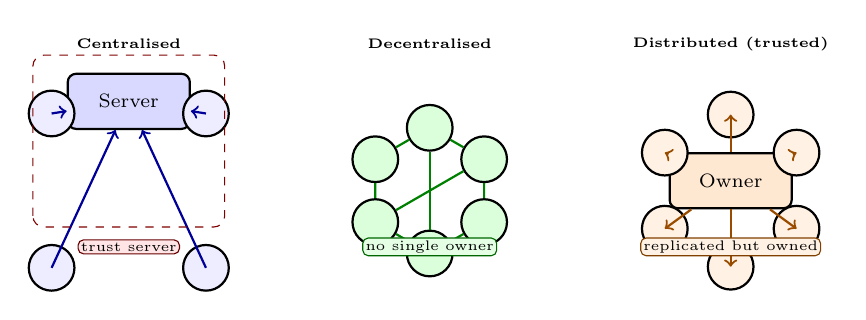
\begin{tikzpicture}[scale=0.84, every node/.style={font=\scriptsize},
  srv/.style={draw,rounded corners=3pt,minimum width=1.55cm,minimum height=0.70cm,align=center,thick},
  cli/.style={draw,circle,minimum size=0.58cm,inner sep=0pt,thick}]
% Centralised
\begin{scope}[xshift=-4.55cm]
  \node[font=\tiny\bfseries] at (0,2.22) {Centralised};
  \node[srv,fill=blue!15] (s) at (0,1.35) {Server};
  \foreach \a in {135,45,-45,-135} {\node[cli,fill=blue!7] at (\a:1.65) {};}
  \foreach \a in {135,45,-45,-135} {\draw[->,thick,blue!60!black] (\a:1.65) -- (s);}
  \draw[rounded corners=4pt,dashed,red!50!black] (-1.45,-0.55) rectangle (1.45,2.05);
  \node[font=\tiny,fill=red!10,draw=red!40!black,rounded corners=2pt,inner sep=1pt] at (0,-0.85) {trust server};
\end{scope}
% Decentralised
\begin{scope}[xshift=0cm]
  \node[font=\tiny\bfseries] at (0,2.22) {Decentralised};
  \foreach \i/\a in {0/90,1/30,2/-30,3/-90,4/-150,5/150} {
    \node[cli,fill=green!14] (n\i) at (\a:0.95) {};}
  \foreach \i in {0,...,5} {\pgfmathtruncatemacro{\j}{mod(\i+1,6)}\draw[thick,green!50!black] (n\i) -- (n\j);}
  \draw[thick,green!50!black] (n0)--(n3); \draw[thick,green!50!black] (n1)--(n4);
  \node[font=\tiny,fill=green!10,draw=green!40!black,rounded corners=2pt,inner sep=1pt] at (0,-0.85) {no single owner};
\end{scope}
% Distributed trusted
\begin{scope}[xshift=4.55cm]
  \node[font=\tiny\bfseries] at (0,2.22) {Distributed (trusted)};
  \node[srv,fill=orange!18] (o) at (0,0.15) {Owner};
  \foreach \a in {90,30,-30,-90,-150,150} {\node[cli,fill=orange!10] at (\a:1.15) {};}
  \foreach \a in {90,30,-30,-90,-150,150} {\draw[->,thick,orange!60!black] (o) -- (\a:1.15);}
  \node[font=\tiny,fill=orange!10,draw=orange!50!black,rounded corners=2pt,inner sep=1pt] at (0,-0.85) {replicated but owned};
\end{scope}
\end{tikzpicture}
\caption{Three replication stories. Only the middle gives every node equal authority. Blockchain adds hash-linking (next figure) so copies can be cross-checked without trusting any one replica. Colour groups trust (blue central, green decentralised, orange owner-replicated).}
\label{fig:topologies}
\end{figure}

% ============================================================
\section{Hash Functions and the Chain}\label{sec:hash-chain}
A \emph{hash function} $H:\{0,1\}^*\to\{0,1\}^{256}$ maps any string to a fixed 256-bit fingerprint. We need:

\begin{definition}[Hash security]\label{def:hash-sec}
$H$ is (i) \emph{preimage resistant}: given $y$, hard to find $x$ with $H(x)=y$; (ii) \emph{second-preimage resistant}: given $x$, hard to find $x'\ne x$ with $H(x')=H(x)$; (iii) \emph{collision resistant}: hard to find any $x\ne x'$ with $H(x)=H(x')$. It is also \emph{avalanche}: flipping one bit of $x$ changes $\approx50\%$ of output bits.
\end{definition}

In practice we use SHA-256. Treat it as a random oracle for reasoning.

A \emph{hash chain} links items $B_0,\dots,B_n$ by storing inside $B_i$ the hash of $B_{i-1}$:
\begin{equation}\label{eq:hash-chain}
h_i = H(B_i \parallel h_{i-1}),\quad h_{-1}:=0^{256},\quad \text{chain head}=h_n .
\end{equation}
To verify, recompute $h_0,\dots,h_n$ and compare the final $h_n$. Tampering with any $B_k$ changes $h_k$ (avalanche) and thus every later $h_{k+1},\dots,h_n$ -- a domino effect.

\begin{figure}[h]\centering
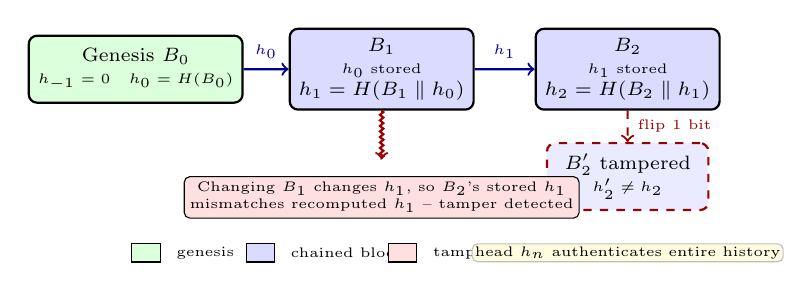
\begin{tikzpicture}[scale=0.88, every node/.style={font=\scriptsize},
  blk/.style={draw,rounded corners=3pt,minimum width=2.05cm,minimum height=0.85cm,align=center,thick}]
\node[blk,fill=green!14] (g) at (0,1.10) {Genesis $B_0$\\ \tiny $h_{-1}=0$\quad $h_0=H(B_0)$};
\node[blk,fill=blue!14] (b1) at (3.55,1.10) {$B_1$\\ \tiny $h_0$ stored\\ $h_1=H(B_1\parallel h_0)$};
\node[blk,fill=blue!14] (b2) at (7.10,1.10) {$B_2$\\ \tiny $h_1$ stored\\ $h_2=H(B_2\parallel h_1)$};
\node[blk,fill=blue!8,dashed,draw=red!60!black] (b2t) at (7.10,-0.45) {$B_2'$ tampered\\ \tiny $h'_2\ne h_2$};
\draw[->,thick,blue!60!black] (g) -- (b1) node[midway,above,font=\tiny] {$h_0$};
\draw[->,thick,blue!60!black] (b1) -- (b2) node[midway,above,font=\tiny] {$h_1$};
\draw[->,thick,red!60!black,dashed] (b2) -- (b2t) node[midway,right,font=\tiny] {flip 1 bit};
\node[draw,fill=red!12,rounded corners=2pt,inner sep=2pt,font=\tiny,align=center] at (3.55,-0.75) {Changing $B_1$ changes $h_1$, so $B_2$'s stored $h_1$\\mismatches recomputed $h_1$ -- tamper detected};
\draw[->,thick,red!60!black,decorate,decoration={zigzag,segment length=2pt,amplitude=0.6pt}] (b1.south) -- (3.55,-0.20);
% legend
\node[draw,fill=green!14,minimum width=0.36cm,minimum height=0.22cm] at (0.15,-1.55) {}; \node[font=\tiny,anchor=west] at (0.45,-1.55) {genesis};
\node[draw,fill=blue!14,minimum width=0.36cm,minimum height=0.22cm] at (1.80,-1.55) {}; \node[font=\tiny,anchor=west] at (2.10,-1.55) {chained block};
\node[draw,fill=red!12,minimum width=0.36cm,minimum height=0.22cm] at (3.85,-1.55) {}; \node[font=\tiny,anchor=west] at (4.15,-1.55) {tamper ripple};
\node[font=\tiny,fill=yellow!12,draw=gray!50,rounded corners=2pt,inner sep=1pt] at (7.10,-1.55) {head $h_n$ authenticates entire history};
\end{tikzpicture}
\caption{Hash chain: each block commits to all previous blocks via nested hashes. Below, tampering with $B_1$ ripples forward (red zigzag). Only the head hash $h_n$ needs to be remembered to verify everything.}
\label{fig:hash-chain}
\end{figure}

\begin{theorem}[Tamper evidence]\label{thm:tamper}
If $H$ is collision resistant, any change to $B_k$ with $k\le n$ is detected by recomputing the chain unless the adversary finds a collision in $H$.
\end{theorem}
\emph{Proof sketch.} Changing $B_k$ changes its hash with overwhelming probability (second-preimage resistance), so recomputed $h_k\ne$ stored $h_k$ in $B_{k+1}$, and inductively all later headers mismatch. \hfill$\square$

\begin{example}[Git vs blockchain]\label{ex:git}
Git commits are hash-chained (each commit hashes its parent). The difference is authority: Git allows history rewriting via force-push; a blockchain's consensus rules forbid rewriting without redoing proof-of-work or acquiring stake, which we formalise in Ch.~2.
\end{example}

A runnable hash chain in Python makes this concrete.

\begin{lstlisting}[language=Python]
import hashlib, json

def H(x: bytes) -> str:
    return hashlib.sha256(x).hexdigest()

def hash_block(data, prev_hash):
    payload = json.dumps(data, sort_keys=True).encode() + prev_hash.encode()
    return H(payload)

# Build chain B0 -> B1 -> B2
chain = []
prev = "0"*64
for data in [{"tx":"Alice->Bob 10"}, {"tx":"Bob->Carol 5"}, {"tx":"Carol->Dave 2"}]:
    h = hash_block(data, prev)
    chain.append((data, prev, h))
    prev = h
    print(data, "prev=", prev[:10]+"...", "hash=", h[:12]+"...")

# Verify
def verify(chain):
    prev = "0"*64
    for data, stored_prev, stored_h in chain:
        assert stored_prev == prev, "prev mismatch -- tamper!"
        assert stored_h == hash_block(data, prev), "hash mismatch!"
        prev = stored_h
    return True

print("verify:", verify(chain))
# Tamper: flip one character in B1
chain[1] = ({"tx":"Bob->Carol 5000"}, chain[1][1], chain[1][2])
try: verify(chain)
except AssertionError as e: print("tamper detected:", e)
\end{lstlisting}

% ============================================================
\section{Anatomy of a Block}\label{sec:block-anatomy}
A block bundles many transactions for efficiency. Splitting \emph{header} (small, hash-linked) from \emph{body} (large, Merkle-committed) lets light clients verify inclusion with $O(\log n)$ hashes (Ch.~5).

\begin{figure}[h]\centering
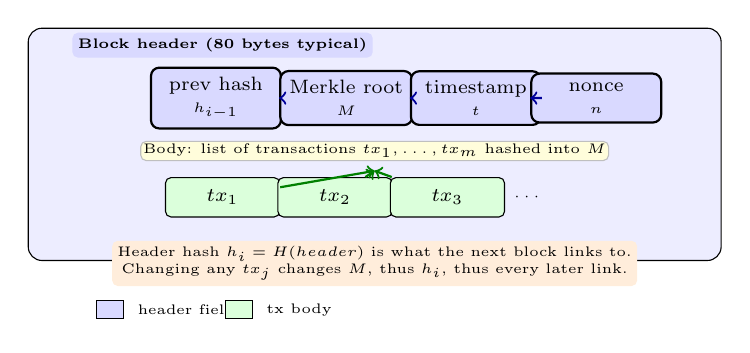
\begin{tikzpicture}[scale=0.84, every node/.style={font=\scriptsize},
  hdr/.style={draw,rounded corners=3pt,fill=blue!15,minimum width=1.65cm,minimum height=0.60cm,align=center,thick},
  tx/.style={draw,rounded corners=2pt,fill=green!14,minimum width=1.45cm,minimum height=0.50cm,align=center}]
\node[draw,rounded corners=5pt,fill=blue!7,minimum width=8.8cm,minimum height=2.95cm] (box) at (4.15,1.05) {};
\node[font=\tiny\bfseries,fill=blue!15,rounded corners=2pt,inner sep=2pt] at (1.85,2.55) {Block header (80 bytes typical)};
\node[hdr] (ph) at (1.75,1.75) {prev hash\\ \tiny $h_{i-1}$};
\node[hdr] (mr) at (3.72,1.75) {Merkle root\\ \tiny $M$};
\node[hdr] (ts) at (5.68,1.75) {timestamp\\ \tiny $t$};
\node[hdr] (no) at (7.50,1.75) {nonce\\ \tiny $n$};
\draw[->,thick,blue!60!black] (ph)--(mr); \draw[->,thick,blue!60!black] (mr)--(ts); \draw[->,thick,blue!60!black] (ts)--(no);
\node[font=\tiny,fill=yellow!14,draw=gray!50,rounded corners=2pt,inner sep=1pt,align=center] at (4.15,0.95) {Body: list of transactions $tx_1,\dots,tx_m$ hashed into $M$};
\node[tx] (t1) at (1.85,0.25) {$tx_1$}; \node[tx] (t2) at (3.55,0.25) {$tx_2$}; \node[tx] (t3) at (5.25,0.25) {$tx_3$}; \node[font=\tiny] at (6.45,0.25) {$\cdots$};
\draw[->,thick,green!50!black] (t1) -- (4.15,0.65); \draw[->,thick,green!50!black] (t2) -- (4.15,0.65); \draw[->,thick,green!50!black] (t3) -- (4.15,0.65);
\node[font=\tiny,align=center,fill=orange!14,rounded corners=2pt,inner sep=2pt] at (4.15,-0.75) {Header hash $h_i=H(\text{header})$ is what the next block links to.\\ Changing any $tx_j$ changes $M$, thus $h_i$, thus every later link.};
% legend
\node[draw,fill=blue!15,minimum width=0.34cm,minimum height=0.20cm] at (0.15,-1.45) {}; \node[font=\tiny,anchor=west] at (0.42,-1.45) {header field};
\node[draw,fill=green!14,minimum width=0.34cm,minimum height=0.20cm] at (2.10,-1.45) {}; \node[font=\tiny,anchor=west] at (2.37,-1.45) {tx body};
\end{tikzpicture}
\caption{Block anatomy: a tiny header commits to a large body via the Merkle root. Light clients store only headers yet can verify any transaction with a Merkle proof.}
\label{fig:block-anatomy}
\end{figure}

\begin{lstlisting}[language=Python]
import hashlib, struct, time
def sha256d(b: bytes) -> bytes:
    return hashlib.sha256(hashlib.sha256(b).digest()).digest()
# Simplified header serialisation (Bitcoin-like)
def header_bytes(prev_hash_hex, merkle_hex, timestamp, nonce):
    return bytes.fromhex(prev_hash_hex)[::-1] + bytes.fromhex(merkle_hex)[::-1] \
           + struct.pack("<II", timestamp, nonce)
prev = "00"*32
merkle = hashlib.sha256(b"tx1|tx2|tx3").hexdigest()
hdr = header_bytes(prev, merkle, int(time.time()), 42)
print("header hash:", sha256d(hdr)[::-1].hex()[:16]+"...")
\end{lstlisting}

% ============================================================
\section{Exercises}\label{sec:ch01-exercises}
\begin{enumerate}[label=E1.\arabic*, leftmargin=*, itemsep=0.6em]
    \item \textbf{Avalanche drill.} Take any sentence, compute SHA-256, flip one bit, recompute. Count differing bits. Repeat 5 times and report the distribution. Why does this matter for tamper evidence?
    \item \textbf{Chain surgery.} Given a 4-block chain, you tamper $B_2$. Which stored hashes become invalid? Must you recompute only $h_2$ or all of $h_2,\dots,h_4$ to hide the change? Relate to collision resistance.
    \item \textbf{Git vs chain.} Explain in one paragraph how Git's hash chain differs from a blockchain's regarding authority to rewrite history. What would Git need to become a blockchain?
    \item \textbf{Header/body split.} A light client stores only 80-byte headers for a chain of $10^6$ blocks. Estimate storage vs a full node with 1\,MB bodies. How does a Merkle proof let the light client verify a transaction without the body?
    \item \textbf{Trust without trust.} A naive design stores ``page number'' links instead of hash links. Show an explicit tampering that page numbers miss but hash links catch. Generalise to why content addressing is essential for decentralisation.
\end{enumerate}

\section*{Chapter Notes}
Nakamoto's Bitcoin whitepaper (2008) introduced the hash chain plus proof-of-work. For hash functions see Katz--Lindell, \emph{Introduction to Modern Cryptography}, Ch.~5. Merkle trees (1979) are detailed in Ch.~5. Narayanan et al., \emph{Bitcoin and Cryptocurrency Technologies} (Princeton, 2016) gives the gentlest full-stack introduction; Buterin's Ethereum whitepaper (2013) extends the model to state machines.
% End Ch01
